\documentclass[11pt,a4paper]{article}

% ---------------------------------------------------------
% Packages
% ---------------------------------------------------------

\usepackage[margin=2.2cm]{geometry}

\usepackage[T1]{fontenc}
\usepackage[utf8]{inputenc}
\usepackage{lmodern}
\usepackage{microtype}

\usepackage{graphicx}
\usepackage{float}

\usepackage{booktabs}
\usepackage{longtable}
\usepackage{array}
\usepackage{tabularx}
\usepackage{multirow}

\usepackage{xcolor}

\usepackage{amsmath}
\usepackage{amssymb}

\usepackage{siunitx}

\usepackage{enumitem}

\usepackage{caption}
\usepackage{subcaption}

\usepackage[numbers,sort&compress]{natbib}

\usepackage[most]{tcolorbox}

\usepackage{hyperref}

% Compact and configurable table of contents
\usepackage{tocloft}


% ---------------------------------------------------------
% Formatting
% ---------------------------------------------------------

\setlength{\parindent}{0pt}
\setlength{\parskip}{0.65em}

\setlist[itemize]{
    leftmargin=*,
    itemsep=0.25em,
    topsep=0.25em
}

\setlist[enumerate]{
    leftmargin=*,
    itemsep=0.25em,
    topsep=0.25em
}

\hypersetup{
    colorlinks=true,
    linkcolor=blue,
    urlcolor=blue,
    citecolor=blue
}

\sisetup{
    round-mode=places,
    round-precision=3,
    detect-all=true
}


% ---------------------------------------------------------
% Table of contents formatting
% ---------------------------------------------------------

% Number subsubsections in the report, but only show sections
% and subsections in the table of contents.
\setcounter{secnumdepth}{3}
\setcounter{tocdepth}{2}

% Make TOC compact enough to remain on one page.
\setlength{\cftbeforesecskip}{2pt}
\setlength{\cftbeforesubsecskip}{1pt}


% ---------------------------------------------------------
% Helper commands
% ---------------------------------------------------------

\definecolor{accentblue}{RGB}{21,96,130}

\newcommand{\placeholder}[1]{%
    \textcolor{accentblue}{\textit{[#1]}}%
}

\newcommand{\todo}[1]{%
    \textcolor{red}{\textbf{[TODO: #1]}}%
}

\newcommand{\code}[1]{%
    \texttt{\detokenize{#1}}%
}


% ---------------------------------------------------------
% Report metadata
% ---------------------------------------------------------

\title{
    \large
    LLM-Based Detection and Revision of Questionnaire Items
}

\author{
    Abdul Samad Najm\\
    \small {Ludwig Maximilian University of Munich / Statistics and Data Science / Seminar}
}

% =========================================================
% DOCUMENT
% =========================================================

\begin{document}

\maketitle


% =========================================================
% ABSTRACT
% Target: approximately 180--250 words
% =========================================================

\begin{abstract}
Questionnaire defects can affect how respondents understand a question, retrieve
information, form a judgement, and map that judgement onto the available response
options. Large language models (LLMs) could support questionnaire review, but useful
automated appraisal requires more than identifying isolated flaws: a system should
also preserve acceptable items, recover multiple independently supported defects, and
revise problematic items without changing the intended construct. This study evaluates 
locally deployed large language models on an expert-reviewed
   benchmark of 200 questionnaire items covering 16 defect categories, including clean, 
   single-defect, and multi-defect cases, with evaluation of both defect detection and 
   construct-preserving revision. A simple checker--reviser pipeline is compared with a 
   role-separated orchestrated workflow under three prompt conditions: a zero-shot taxonomy 
   codebook, additional operational rules, and family-spanning few-shot demonstrations. 
   Performance varied substantially across models, prompting strategies, and architectures. 
   Qwen achieved the strongest overall results, with P2 orchestration reaching a micro-F1 of 
   0.563, an exact label-set match of 0.430, and a clean-item false-positive rate of 0.050. 
   The baseline generally achieved higher recall and broader multi-label coverage, but also 
   produced more unsupported labels, whereas orchestration was more selective and preserved 
   clean items more reliably. Few-shot calibration improved selected 
   response-option and scale decisions, but gains were uneven across models and defect categories. 
   Thinking mode improved detection among successfully completed outputs, but reduced structured-output 
   reliability. Overall, the results show that LLM-based questionnaire appraisal involves a trade-off 
   between defect coverage, restraint, revision quality, and operational reliability, and that structured 
   prompting and orchestration can improve selected aspects of performance without yet providing 
   consistently reliable end-to-end automation.
\end{abstract}


% =========================================================
% TABLE OF CONTENTS
% =========================================================

\newpage

\tableofcontents

\newpage


% =========================================================
% 1. INTRODUCTION
% Replace the existing Introduction with this section.
% =========================================================

\section{Introduction}
\label{sec:introduction}

Poorly designed survey questions can distort the data they are intended to collect.
Problems may arise from the wording of the question itself or from the response
options through which respondents are asked to express an answer.  
Classic questionnaire-design examples illustrate how easily such
problems can arise. Saris and Gallhofer, for instance, discuss an item that asks
respondents to evaluate the European Parliament and the European Commission using
a single response. Because a respondent may judge the two institutions differently,
the item combines distinct evaluations and is therefore double-barreled. They also
discuss the seemingly straightforward question ``What is the best book you read last
year?'', which presupposes that the respondent read at least one book during the
specified period~\cite{saris2014design}. Such flaws are easy to introduce but can
prevent respondents from answering as intended. Even minor design choices can shape
how respondents interpret a question and formulate an answer; when the cognitive
burden becomes too high, they may satisfice rather than engage carefully with the
task~\cite{tourangeau2000psychology,krosnick1991response}.

Established approaches for identifying these problems include expert review,
questionnaire appraisal, cognitive interviewing, behaviour coding, respondent
debriefing, and field pretesting \cite{presser2004methods}. These procedures provide
different kinds of evidence and remain important for questionnaire development, but
they also require methodological expertise, appropriate participants, and iterative
review. An automated system could therefore be useful as an early screening and
revision aid, particularly when specialist survey-methods expertise is not immediately
available. Such assistance should complement rather than replace expert and
respondent-based evaluation, since problems that emerge during actual interpretation
and response may not be visible from the questionnaire text alone.

Against this background, we investigate whether locally deployed LLMs can support
questionnaire review by distinguishing acceptable items from problematic ones,
identifying the specific design problems present, and proposing targeted revisions
without changing what the question is intended to measure. The evaluation uses an
expert-reviewed benchmark of 200 questionnaire items under a closed 16-label
taxonomy and evaluates both defect detection and construct-preserving revision.
Two ways of organizing the same underlying LLM are compared: a simple
checker--reviser workflow and a role-separated workflow that divides detection,
planning, revision, and validation across specialized calls. The study further
examines whether performance changes when the models receive increasingly explicit
guidance, moving from taxonomy definitions to operational rules and then to
few-shot examples.

The study is guided by three research questions:
\begin{tcolorbox}[
    colback=blue!1!white,
    colframe=accentblue!90!black,
    title=Research Questions,
    fonttitle=\bfseries,
    coltitle=white,
    boxrule=0.7pt,
    arc=2mm
]
\begin{description}[
    style=nextline,
    leftmargin=1.7cm,
    labelwidth=1.2cm,
    font=\bfseries,
    itemsep=5pt
]
    \item[RQ1:] How accurately can locally deployed LLMs distinguish acceptable
    questionnaire items from items containing one or more taxonomy-defined defects?

    \item[RQ2:] How does a role-separated workflow compare with a simpler
    checker--reviser workflow in defect detection, clean-item preservation, and
    construct-preserving revision?

    \item[RQ3:] How does increasingly explicit prompt guidance affect detection and
    revision performance, and are these effects consistent across defect families?
\end{description}
\end{tcolorbox}


\section{Related Work}
\label{sec:related-work}

Prior work relevant to this study can be organized around two related questions:
how questionnaire problems can be identified before data collection, and how recent
LLM-based methods extend such appraisal toward automated critique and revision.
The first line of work establishes explicit principles and tools for questionnaire
evaluation, while the second examines how reliably LLMs can apply related judgments
without continuous expert intervention.

\subsection{Structured and Computer-Assisted Questionnaire Appraisal}
\label{subsec:structured-appraisal}

Questionnaire evaluation methods differ in both the problems they target and the
evidence on which their judgments are based. Expert appraisal evaluates an
instrument against known design principles, whereas cognitive interviewing,
behaviour coding, and field pretesting provide progressively more direct evidence
about how respondents interact with a question
\cite{presser2004methods}. Saris and Gallhofer provide a broader framework for
questionnaire design in which the measured concept, formulation of the request,
response alternatives, scale properties, and overall survey-item structure are
treated as consequential design choices \cite{saris2014design}. Their discussion
covers problems such as double-barreled requests, implicit assumptions, complex
formulations, incomplete or overlapping response alternatives, mismatches between
the request and its response categories, and choices in scale construction. These
principles are relevant to the present study beyond their later implementation in
SQP and provide methodological grounding for several defect mechanisms examined
in the benchmark.

Structured and computer-assisted approaches operationalize these principles in
different ways. The Question Appraisal System (QAS-99) organizes expert appraisal
into explicit decisions concerning potential questionnaire problems
\cite{willis1999qas}. QUAID instead provides automated screening for selected
comprehension risks, including unfamiliar or vague terms, ambiguous noun phrases,
complex syntax, and working-memory demands \cite{graesser2006quaid}. The Survey
Quality Predictor (SQP) addresses a different target: it uses coded characteristics
of survey questions and evidence from multitrait--multimethod experiments to
predict reliability, validity, and overall measurement quality
\cite{saris2014design}. These systems therefore range from structured diagnosis of
potential problems to automated comprehension screening and prediction of expected
measurement quality.

The methods should not be treated as interchangeable. Maitland and Presser compared
QUAID, SQP, expert review, QAS, and cognitive interviewing against problems observed
under more typical survey conditions and found that the approaches identified
partly different problems and differed between subjective and objective questions
\cite{maitland2018question}. Their results support the use of multiple forms of
evidence rather than treating any single appraisal procedure as sufficient. For the
present study, this distinction motivates viewing automated LLM appraisal as an
early screening and revision layer whose outputs remain subject to methodological
evaluation rather than as a replacement for human or respondent-based testing.


\subsection{LLMs for Questionnaire Design, Pretesting, and Appraisal}
\label{subsec:llm-questionnaires}

Recent LLM research has first examined whether models can assist with questionnaire
generation and revision. Adhikari et al.\ combine questionnaire generation,
LLM-simulated pretesting, review, and cultural adaptation within a single development
pipeline \cite{adhikari2025exploring}. Their evaluations suggest that LLM-generated
or adapted wording can be useful, while additional simulated refinement does not
necessarily improve an item and can sometimes increase its complexity. Fuchs et al.\
similarly show that the quality of LLM-generated survey items varies across models
and prompting strategies \cite{fuchs2026ai}. Taken together, this work indicates
that LLMs can support questionnaire construction, but additional model calls or more
elaborate prompting cannot be assumed to improve questionnaire quality.

A second line of work focuses more directly on identifying problems in existing
questions. Metheney and Yehle examine free-text LLM critiques and find that the
number and type of reported problems vary with model and prompting condition
\cite{metheney2025generative}. Sturgis et al.\ evaluate LLMs against deliberately
embedded questionnaire flaws and clean control items, showing that guided prompting
can detect a substantial proportion of known problems while still exhibiting
model- and prompt-dependent differences \cite{sturgis2026llms}. Roberts et al.\
move further toward structured appraisal by comparing LLM-based QAS-99 decisions
with expert and novice human coders; agreement varies substantially by appraisal
category, and the models identify fewer problems than the questionnaire-design
expert \cite{roberts2026survey}. Across these studies, LLM performance is therefore
not uniform across models, prompts, or types of questionnaire problem.

The existing literature establishes that LLMs can generate questionnaire items,
provide useful critiques, simulate selected pretesting activities, and apply
structured appraisal criteria. What is less well established is whether the same
system can reliably combine several requirements: recognize when no intervention is
needed, recover all independently supported defects when several occur together,
avoid unsupported diagnoses, and convert the detected problems into minimal
construct-preserving revisions. The present study evaluates these requirements
jointly under one controlled benchmark while also comparing prompt guidance and
runtime organization. A more detailed comparison with selected prior systems and
studies is provided in Appendix~\ref{app:benchmark}.
% =========================================================
% 3. BENCHMARK AND TASK DESIGN
% Target: ~1.25--1.5 pages
% =========================================================
\section{Benchmark and Task Design}
\label{sec:benchmark}

\subsection{Questionnaire-Defect Taxonomy}
\label{subsec:taxonomy}

The benchmark uses a closed 16-label taxonomy of questionnaire-design defects
developed for the present study. The taxonomy operationalizes questionnaire-design
problems and principles discussed by Saris and Gallhofer~\cite{saris2014design},
while the specific labels and decision boundaries were defined for consistent
annotation and evaluation in this study. Let
$\mathcal{T}$ denote this taxonomy and $Y_i\subseteq\mathcal{T}$ the gold label
set for item $i$. A clean item has $Y_i=\varnothing$; a flawed item has one or
more labels. Multiple labels are assigned only when each defect has separate
visible evidence, fixing either defect alone would leave the other unresolved,
and each would independently justify a repair. This independent-label rule
prevents stylistic preferences or correlated symptoms from becoming additional
gold labels.

Table~\ref{tab:taxonomy} maps the labels to the five repair families used by the
orchestrated system. Counts are label appearances, not unique items; a
multi-label item contributes once for every applicable label.

\begin{table}[H]
\centering
\caption{Taxonomy labels, repair families, and gold-label appearances.}
\label{tab:taxonomy}
\small
\begin{tabularx}{\textwidth}{p{0.20\textwidth}Xr}
\toprule
\textbf{Repair family} & \textbf{Taxonomy labels} & \textbf{Instances} \\
\midrule
Wording clarity
& \code{leading_question}, \code{loaded_question}, \code{recall_error},
  \code{vague_ambiguous}, \code{negative_wording} & 65 \\
Construct alignment
& \code{double_barreled} & 12 \\
Bias sensitivity
& \code{sensitive_topic_direct}, \code{social_desirability} & 24 \\
Questionnaire format
& \code{open_closed_mismatch} & 12 \\
Response options and scale
& \code{agree_disagree_scale}, \code{unbalanced_scale},
  \code{incomplete_options}, \code{non_exclusive_options},
  \code{missing_scale_labels}, \code{too_many_scale_points},
  \code{polarity_mismatch} & 93 \\
\midrule
\textbf{Total} & \textbf{16 taxonomy labels} & \textbf{206} \\
\bottomrule
\end{tabularx}
\end{table}

Several of these distinctions correspond to questionnaire-design problems discussed
by Saris and Gallhofer, including double-barreled requests, implicit assumptions,
response-category coverage and exclusivity, scale construction, and
stem--response compatibility~\cite{saris2014design}.

To connect defect detection with revision, the 16 taxonomy labels are organized
into five specialist families according to the type of repair they require.
Taxonomy labels remain the units of annotation and evaluation, whereas specialist
families determine which role is responsible for revising an item.

\begin{minipage}{\linewidth}
\textbf{Wording clarity.}
This family covers defects that affect how respondents interpret the question
stem. \code{leading_question} identifies wording that steers respondents toward
a particular answer, whereas \code{loaded_question} identifies an unverified
presupposition. \code{recall_error} concerns demands that exceed reasonable
memory capabilities, while \code{vague_ambiguous} captures unclear or
underspecified meaning. \code{negative_wording} covers difficult negation or
reverse wording.
\end{minipage}

\textbf{Construct alignment.}
This family contains \code{double_barreled}, which applies when a single response
is required for two separable constructs that respondents could evaluate
differently.

\textbf{Bias sensitivity.}
This family distinguishes two sources of bias.
\code{sensitive_topic_direct} concerns insufficient protection when asking about
sensitive matters, whereas \code{social_desirability} concerns wording that
pressures respondents toward a socially approved answer.

\textbf{Questionnaire format.}
This family contains \code{open_closed_mismatch}, which identifies an
incompatibility between the response task requested by the question stem and the
format of the supplied response options.

\textbf{Response options and scale.}
This family covers defects in how answers are represented.
\code{agree_disagree_scale} identifies the use of generic agreement options when
an item-specific scale is required. \code{incomplete_options} concerns inadequate
response coverage, \code{non_exclusive_options} concerns overlapping categories,
and \code{unbalanced_scale} concerns asymmetric coverage of an ordered continuum.
The remaining labels address scale construction: \code{missing_scale_labels}
concerns interpretability, \code{too_many_scale_points} concerns unjustified
precision, and \code{polarity_mismatch} concerns disagreement between the
question stem and the direction of the response scale.

The five families contain five, one, two, one, and seven labels, respectively.
This unequal structure reflects similarities in the required repair operations
rather than an attempt to balance the groups. Their benchmark frequencies also
vary substantially, ranging from 12 to 93 label appearances. Family-level scores
should therefore be interpreted with their denominators and alongside the
corresponding per-label results.

\subsection{Final 200-Item Gold Benchmark}
\label{subsec:gold-benchmark}

The empirical evaluation uses an expert-reviewed gold benchmark of 200 questionnaire items. The benchmark was constructed through a human-directed, LLM-assisted process in which frontier large language models supported item drafting, diversification, and construct-preserving revision. The taxonomy, benchmark design, annotation criteria, and final labels were defined and reviewed by the researchers. The resulting benchmark therefore serves as an expert-reviewed reference standard for evaluating defect detection and questionnaire revision.

\begin{table}[H]
\centering
\caption{Composition of the final expert-reviewed benchmark.}
\label{tab:benchmark-composition}
\small
\begin{tabular}{lr}
\toprule
\textbf{Property} & \textbf{Count}\\
\midrule
Total questionnaire items & 200\\
Clean controls & 40\\
Flawed items & 160\\
Single-label flawed items & 115\\
Multi-label flawed items & 45\\
Taxonomy labels & 16\\
Total gold-label appearances & 206\\
\bottomrule
\end{tabular}
\end{table}

The 40 clean controls contain no independently supported defect under the
taxonomy. Their inclusion is essential because a questionnaire-review system
must do more than detect problematic items: it must also recognize when no
intervention is required. These items therefore make it possible to measure
false-positive detection and unnecessary revision, or \emph{overcorrection}.
For clean controls, the reference revision preserves the original question and
response options unchanged.

The 160 flawed items are divided into 115 single-label and 45 multi-label
cases. A single-label item isolates one principal defect mechanism and is useful
for determining whether a model can distinguish closely related taxonomy
categories. A multi-label item contains two or more defects that are
independently supported by visible evidence. In such cases, correcting only one
defect is insufficient because another measurement problem remains. These items
therefore test whether a system can recover a complete label set and coordinate
a revision that addresses all applicable problems while preserving unaffected
parts of the item. Because multi-label items contribute once to the count of
each applicable category, the 200 items contain 206 gold-label appearances.

The benchmark spans 14 substantive domains, nine response formats, and three
approximately balanced difficulty groups; detailed topic counts are reported in
Appendix~\ref{app:benchmark}.


Taken together, the benchmark supports three complementary forms of
evaluation. Clean controls test restraint, single-label items test
category-specific discrimination, and multi-label items test completeness and
coordinated repair. Its breadth of topics, response formats, and difficulty
levels further tests whether questionnaire-defect detection transfers across
different substantive contexts rather than depending on one domain or a small
set of surface patterns. At the same time, the benchmark remains a controlled,
LLM-assisted and expert-reviewed collection rather than a representative sample
of all questionnaires used in practice; this limitation is considered in
Section~\ref{subsec:limitations}.



\subsection{Detection and Revision Tasks}
\label{subsec:task-definition}

For item $i$, the benchmark input is $x_i=(q_i,O_i)$, with question $q_i$
and ordered options $O_i$. Only these fields enter the initial checker or router.
Downstream roles may receive runtime-generated issues or plans, but never IDs,
gold labels, expected revisions, target concepts, topics, metadata, or review
notes; direct annotation and revision leakage is therefore excluded.

The detection task is multi-label classification,
\[
    \widehat{Y}_i=f(q_i,O_i), \qquad \widehat{Y}_i\subseteq\mathcal{T}.
\]
The model must return the empty set for a clean item and every independently
supported label for a flawed item; omissions and unsupported additions are both
errors. The revision task produces $(\widehat{q}_i,\widehat{O}_i)$ and must fix
all detected defects with minimal change while preserving the intended construct.
A multi-label repair is incomplete if one defect remains, whereas a clean item
must be returned exactly unchanged. Each flawed row has one reference revision for reproducible comparison;
semantic editing metrics supplement the strict reference-based measures.


\section{Methodology}
\label{sec:methodology}

The study varies two components independently: the runtime architecture and the
prompt treatment. The baseline and orchestrated architectures are each evaluated
with the additive P0--P2 prompt conditions. Within an experimental run, the same
LLM checkpoint is used for every role; orchestration changes the division of
responsibilities and sequence of calls rather than combining different models.

\begin{figure}[H]
    \centering
    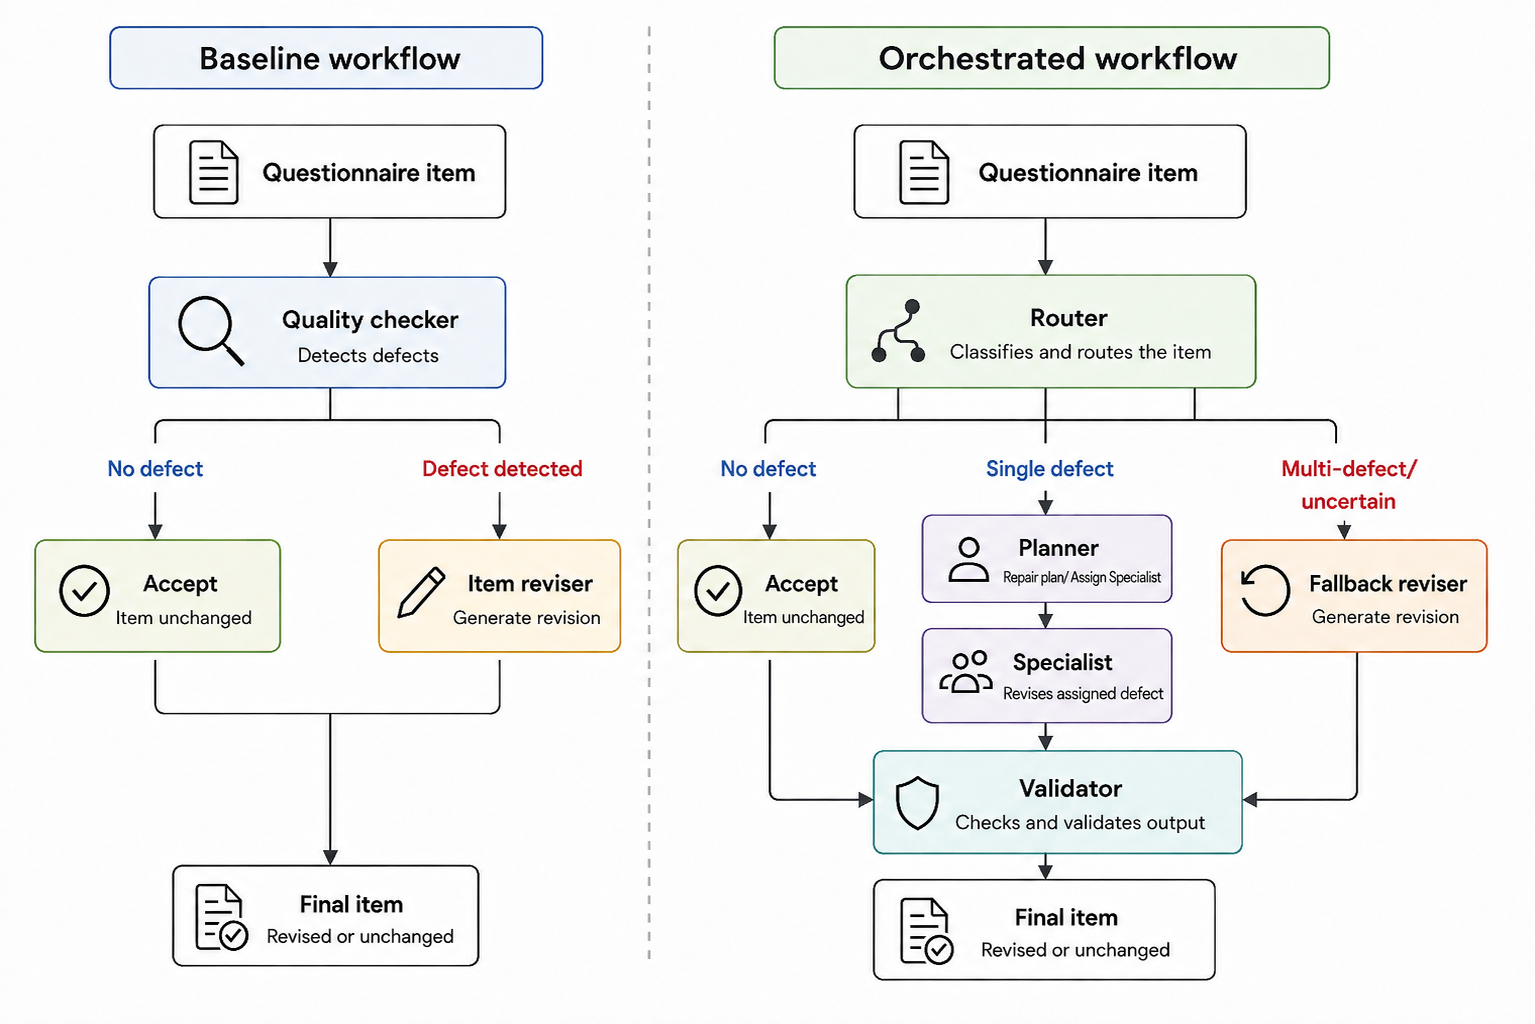
\includegraphics[width=0.82\textwidth]{high-level-architecture-comparison.png}
    \caption{High-level comparison of the baseline and orchestrated workflows.
    Detailed role-level control flow is provided in
    Appendix~\ref{app:architecture}, Figures~\ref{fig:orchestration} and
\ref{fig:orchestration-agents}.}
    \label{fig:architecture-overview}
\end{figure}

% ---------------------------------------------------------
\subsection{Baseline Architecture}
\label{subsec:baseline}

The baseline architecture consists of an LLM-based quality checker followed,
when necessary, by an LLM-based item reviser. For an item $x=(q,O)$, where $q$
is the question and $O$ the ordered response-option list, the checker predicts
all independently supported taxonomy defects and returns their categories,
item-specific severity, explanations, and evidence. It does not revise the
item.

The next step depends on the checker output:
\[
    \text{Item}\rightarrow\text{Quality Checker}\rightarrow
    \begin{cases}
        \text{preserve unchanged}, & \text{no detected defect},\\
        \text{general Item Reviser}, & \text{one or more detected defects}.
    \end{cases}
\]
The reviser receives the original item and the detected issues and returns a
revised question, response options, revision notes, and a changed flag. When no
issue is detected, revision is skipped and the original item is copied to the
final output. The baseline therefore provides a simple reference architecture
without explicit routing, specialist assignment, or post-revision validation.

% ---------------------------------------------------------
\subsection{Orchestrated Architecture}
\label{subsec:orchestration}

The orchestrated architecture separates detection, planning, repair, and
validation into role-specific LLM calls. Its control flow branches after the
router:
\[
    \text{Item}\rightarrow\text{Router}\rightarrow
    \begin{cases}
        \text{unchanged item}\rightarrow\text{Validator},
        & \text{clean accept path},\\
        \text{Planner}\rightarrow\text{Specialist}\rightarrow\text{Validator},
        & \text{clear single-label path},\\
        \text{Fallback Reviser}\rightarrow\text{Validator},
        & \text{multi-label or uncertain path}.
    \end{cases}
\]

\paragraph{Routing and planning.}
The router returns \code{accept}, \code{revise}, or \code{fallback}, together
with taxonomy labels, evidence, a confidence score, and a recommended route. A
single clearly supported defect is mapped to its canonical specialist family.
The default policy instead uses fallback for multiple labels, mixed families,
confidence below 0.7, contradictory outputs, unsupported labels, or ambiguous
routes. The planner is invoked only on the specialist path. It converts the
router's fixed issue set into a minimal repair plan but may neither change the
labels nor rewrite the item.

\paragraph{Specialists and fallback.}
The five specialist roles correspond to the repair families defined above:
wording clarity, response options and scale, construct alignment, bias
sensitivity, and questionnaire format. Each
specialist repairs only its assigned family and must preserve all unrelated
content. The fallback reviser handles multi-label, low-confidence, conflicting,
or otherwise unsafe cases. It coordinates all independently supported repairs
when the evidence is clear, but may preserve the original item when a speculative
change would be less safe.

\paragraph{Validation.}
The validator evaluates rather than rewrites. It checks whether the candidate
preserves the construct, fixes every supplied defect, and introduces no new
supported defect. Clean items accepted by the router are also validated in
unchanged form. The possible statuses are \code{pass}, \code{retry},
\code{manual_review}, and \code{failed}. One validator-triggered retry is
permitted; unresolved or unsafe candidates are flagged for manual review.
\code{failed} is reserved for outputs that cannot be evaluated because the
candidate information is missing, malformed, or unusable.

All roles return schema-constrained JSON. Invalid JSON or schema violations
trigger format-repair attempts within the same role; these are separate from
the validator's semantic revision retry.

% ---------------------------------------------------------
\subsection{Prompt Treatments and Revision Contract}
\label{subsec:prompt-treatments}

The prompt conditions are additive:
\[
    \boxed{\mathrm{P0}\subset\mathrm{P1}\subset\mathrm{P2}}.
\]
P1 retains P0 and adds operational procedures, while P2 retains P1 and adds
fixed demonstrations. Separate but corresponding prompt packs are used for the
baseline and orchestrated architectures.

%\paragraph{P0: Zero-shot taxonomy codebook.}
P0 is the zero-shot control. It provides definitions of all 16 labels,
decision boundaries between related categories, an evidence gate, independent
multi-label logic, clean-item preservation, and minimal-revision rules. It
contains no demonstrations and therefore measures performance from the
codebook and task instructions alone.

%\paragraph{P1: Operational response-option and format rules.}
P1 was introduced after preliminary development runs showed weaknesses on
response-option, scale, and questionnaire-format defects. In addition to P0,
it requires the model to identify the response mode and intended dimension or
unit before checking agreement proxies, completeness, mutual exclusivity,
balance, labels, granularity, polarity, count--rate consistency, and
open--closed compatibility. Matching repair procedures require the smallest
supported correction and prohibit routine additions such as ``Other'',
``Don't know'', or refusal options without visible evidence. P1 contains no
few-shot examples, so it isolates the effect of explicit operational guidance.
In the orchestrated pipeline, these additions are concentrated in the router,
fallback reviser, response-options specialist, questionnaire-format specialist,
and validator.

%\paragraph{P2: Family-spanning few-shot calibration.}
P2 retains P1 and adds fixed, role-specific, schema-valid demonstrations. The
examples calibrate detection, revision, routing, fallback restraint, clean-item
preservation, and validation. Every specialist family is represented, but the
examples are not balanced across all 16 individual taxonomy labels:
\[
    \boxed{\text{P2 is family-complete, but not taxonomy-complete.}}
\]

P2 contains 37 fixed, role-specific demonstrations spanning all five specialist
families; the full role-wise distribution is reported in
Appendix~\ref{app:prompt-packs}.

% ---------------------------------------------------------
All prompt conditions treat revision as targeted repair rather than unrestricted
rewriting. The model must correct only independently supported defects while
preserving the construct, population, reference period, response dimension, and
all non-defective wording and option properties. The question or response set
should be changed only where required, clean items must remain unchanged, and no
repair may introduce a new taxonomy-defined problem. For multi-label items,
every independently supported label remains a separate repair obligation.

% ---------------------------------------------------------
\subsection{Thinking-Mode Ablation}
\label{subsec:thinking-method}

A supplementary P2 ablation evaluates the Qwen model's native reasoning, or
``thinking'', mode under both architectures. The prompts and external JSON
contract remain unchanged; only the model's chat-template thinking mechanism is
toggled. When enabled, the internal reasoning segment is removed before the
final response is parsed against the same schema as in the non-thinking
condition. Completion reliability and conditional task performance are reported
separately in Section~\ref{subsec:thinking-results}.


\section{Results and Discussion}
\label{sec:results}
\label{sec:discussion}

The experiments are analyzed descriptively because each condition was run once
with deterministic decoding. The main comparisons therefore concern matched
changes in models, prompt packs, and architectures rather than sampling-based
significance tests. Detection results are reported on the complete benchmark,
whereas revision metrics are computed on the 160 gold-flawed items with valid
reference revisions. Failed items count as missing predictions in detection
metrics and are excluded from semantic revision averages.


% ---------------------------------------------------------
\subsection{Analysis Scope and Completion Reliability}
\label{subsec:analysis-scope}

All 20 non-thinking runs reached all 200 benchmark items. Most also showed high
structured-output reliability: across the twelve non-thinking Qwen runs, only one
item-level failure occurred. Mistral produced ten failures across its four P0
runs, and Gemma produced 17 across its four P0 runs. 

The four thinking-mode runs are treated separately in
Section~\ref{subsec:thinking-results}. Three stopped before all 200 items had
been reached, and all four produced substantial numbers of invalid structured
outputs, mostly because internal reasoning exhausted the available generation
budget before a valid JSON answer was completed. Consequently, their task
metrics are reported only conditionally on successful outputs. Whenever a
thinking result is contrasted with a non-thinking result, the non-thinking
metric is recomputed on exactly the same successful item IDs.


% ---------------------------------------------------------
\subsection{Overall Detection Performance and Cross-Model Patterns}
\label{subsec:overall-results}
\label{subsec:cross-model}

Table~\ref{tab:overall-detection} reports the complete non-thinking end-to-end
results. The strongest complete configuration was Qwen P2 with orchestration,
which achieved micro-F1 $0.563$, exact label-set match $0.430$, and a clean
false-positive rate of $0.050$. Qwen P2 with the baseline architecture achieved
the highest recall, $0.684$, but its lower precision and higher clean
false-positive rate illustrate the baseline's more aggressive labeling
behavior.

\begin{table}[H]
\centering
\caption{End-to-end detection results without thinking. Failed items remain in
         the 200-item denominator and cannot count as exact matches.}
\label{tab:overall-detection}
\scriptsize
\setlength{\tabcolsep}{3.2pt}
\resizebox{\textwidth}{!}{%
\begin{tabular}{lllrrrrrrr}
\toprule
\textbf{Model} & \textbf{Prompt} & \textbf{Architecture}
& \textbf{Precision} & \textbf{Recall} & \textbf{F1}
& \textbf{Exact} & \textbf{Clean FPR} & \textbf{Overcorr.}
& \textbf{Failed} \\
\midrule
Mistral-7B & P0 & Baseline
& 0.178 & 0.146 & 0.160 & 0.125 & 0.750 & 0.525 & 3 \\

Mistral-7B & P0 & Orchestrated
& 0.235 & 0.019 & 0.036 & 0.205 & 0.000 & 0.000 & 1 \\

\addlinespace
Gemma-2-9B & P0 & Baseline
& 0.379 & 0.320 & 0.347 & 0.270 & 0.725 & 0.725 & 0 \\

Gemma-2-9B & P0 & Orchestrated
& 0.383 & 0.150 & 0.216 & 0.305 & 0.075 & 0.125 & 7 \\

\addlinespace
Qwen3.5-9B & P0 & Baseline
& 0.428 & 0.660 & 0.519 & 0.290 & 0.150 & 0.150 & 0 \\

Qwen3.5-9B & P0 & Orchestrated
& 0.795 & 0.340 & 0.476 & 0.370 & 0.050 & 0.050 & 0 \\

Qwen3.5-9B & P1 & Baseline
& 0.413 & 0.636 & 0.501 & 0.280 & 0.075 & 0.075 & 1 \\

Qwen3.5-9B & P1 & Orchestrated
& 0.845 & 0.345 & 0.490 & 0.375 & 0.025 & 0.000 & 0 \\

Qwen3.5-9B & P2 & Baseline
& 0.443 & \textbf{0.684} & 0.538 & 0.270 & 0.175 & 0.150 & 0 \\

Qwen3.5-9B & P2 & Orchestrated
& \textbf{0.845} & 0.422 & \textbf{0.563} & \textbf{0.430}
& 0.050 & 0.050 & 0 \\

\bottomrule
\end{tabular}%
}

\vspace{0.25em}
\begin{minipage}{0.98\textwidth}
\scriptsize
\end{minipage}
\end{table}

At P0, Qwen achieved the strongest performance in both architectures, followed
by Gemma and then Mistral. For the weaker models, orchestration primarily
increased conservatism rather than improving label recognition. Mistral, for
example, produced no false positives on the 40 clean items but recovered only
four of the 206 gold-label appearances. A low clean false-positive rate can
therefore be misleading when it results from broad under-detection. The complete
family-level breakdown is reported in Appendix~\ref{app:detection}.

Conservative routing did not, however, always indicate a failure to detect
defects. In some cases, it correctly prevented unnecessary revision of clean
items. This distinction is illustrated by the following Qwen P2 example:

\begin{quote}
\small

\textbf{Question:} \emph{Some people prefer not to answer questions about
gambling. During the last 12 months, how many times did you gamble with money?}

\medskip
\textbf{Response options:}

0 times\\
1 time\\
2--3 times\\
4--11 times\\
12 or more times\\
Prefer not to answer

\medskip
\textbf{Gold annotation:} Clean item; no taxonomy defect.
\end{quote}

The baseline incorrectly predicted \code{incomplete_options} and
\code{loaded_question} and consequently rewrote the item as a two-part filter
question. By contrast, the orchestrated router detected no defect and preserved
the original item. In this case, orchestration's lower false-positive tendency
reflected appropriate restraint rather than under-detection. Taken together,
these results show that clean-item performance must be interpreted alongside
defect recall: conservative behavior may either preserve a valid item or conceal
a failure to identify genuine defects.


% ---------------------------------------------------------
\subsection{Effects of the P1 and P2 Prompt Packs}
\label{subsec:prompt-results}
\label{subsec:prompt-discussion}

The matched Qwen comparisons in Table~\ref{tab:overall-detection} isolate
prompt-pack effects within each architecture. They show that additional prompt
content was not automatically beneficial. P1 reduced false positives on clean
items, but did not improve overall baseline detection and produced only a small
orchestrated gain. P2 had a clearer effect, particularly under orchestration.
Complete TP, FP, and FN diagnostics are reported in
Appendix~\ref{app:detection}.

\paragraph{P1: Operational rules.}
As shown in Table~\ref{tab:overall-detection}, for the baseline architecture,
P1 reduced F1 from $0.519$ to $0.501$: true positives fell by five, false
positives increased by four, and false negatives increased by five. Its main
benefit was restraint on clean controls, where FPR fell from $0.150$ to $0.075$.
For orchestration, P1 increased precision from $0.795$ to $0.845$ while recall
remained almost unchanged, producing a modest F1 increase from $0.476$ to
$0.490$ and reducing clean FPR to $0.025$.

The operational rules helped selected categories but did not solve the broader
response-option problem. As shown in the per-label results in
Table~\ref{tab:qwen-label-f1}, baseline \code{open_closed_mismatch} F1 improved
from $0.556$ to $0.632$, and \code{unbalanced_scale} improved from $0.250$ to
$0.435$. Conversely, \code{non_exclusive_options} fell from $0.545$ to $0.200$
and \code{polarity_mismatch} from $0.786$ to $0.667$. At the family level,
Table~\ref{tab:qwen-family-f1} shows that response-options-and-scale F1 fell
from $0.488$ to $0.444$ in the baseline and was essentially unchanged under
orchestration ($0.350$ to $0.344$). P1 therefore improved some decision
boundaries and clean-item restraint, but explicit procedures alone did not
yield a general response-option gain.

\paragraph{P2: Few-shot calibration.}
P2 produced the best Qwen F1 in both architectures. Relative to P1, baseline F1
increased from $0.501$ to $0.538$, driven primarily by recall. Under
orchestration, P2 increased true positives from 71 to 87 while adding only
three false positives; recall rose from $0.345$ to $0.422$, F1 from $0.490$ to
$0.563$, and exact match from $0.375$ to $0.430$. Relative to P0, the
orchestrated F1 gain was $0.087$. The few-shot treatment was therefore most
effective when demonstrations were combined with role-specific routing and
repair responsibilities.

The family-level results in Table~\ref{tab:qwen-family-f1} show that this gain
was not uniform. Under orchestration, the largest P2 improvement was in response
options and scale, whose F1 increased from $0.350$ under P0 and $0.344$ under
P1 to $0.507$. Wording clarity also increased to $0.574$. Construct alignment
returned to $0.857$, while questionnaire format remained at $0.400$ and bias
sensitivity declined to $0.634$. In the baseline, P2 reached the highest
construct-alignment F1 ($0.957$) and response-options F1 ($0.504$), but its
questionnaire-format result fell below both P0 and P1. Family-spanning examples
therefore supported broader transfer, but did not make performance uniformly
better across families.

\begin{table}[H]
\centering
\caption{Qwen family-level micro-F1 across prompt packs.}
\label{tab:qwen-family-f1}
\small
\setlength{\tabcolsep}{4.5pt}
\resizebox{\textwidth}{!}{%
\begin{tabular}{llrrrrr}
\toprule
\textbf{Prompt} & \textbf{Architecture}
& \textbf{Wording} & \textbf{Construct} & \textbf{Bias}
& \textbf{Format} & \textbf{Options/scale} \\
\midrule
P0 & Baseline
& 0.469 & 0.917 & 0.682 & 0.556 & 0.488 \\

P0 & Orchestrated
& 0.495 & 0.857 & 0.667 & 0.286 & 0.350 \\

P1 & Baseline
& 0.474 & 0.870 & 0.698 & 0.632 & 0.444 \\

P1 & Orchestrated
& 0.547 & 0.800 & 0.684 & 0.400 & 0.344 \\

P2 & Baseline
& 0.503 & 0.957 & 0.698 & 0.471 & 0.504 \\

P2 & Orchestrated
& 0.574 & 0.857 & 0.634 & 0.400 & 0.507 \\
\bottomrule
\end{tabular}%
}
\end{table}

Complete per-label F1 values are reported in
Appendix~\ref{app:detection} (Table~\ref{tab:qwen-label-f1}). P2 orchestration
produced especially strong gains for \code{leading_question} and
\code{loaded_question}, and it improved several response-option and scale
defects, including agreement proxies, incomplete option sets, missing scale
labels, excessive scale points, and polarity mismatches.

The improved distinction between leading and loaded wording is visible in one
representative item. The benchmark question was:

\begin{quote}
\small
\textbf{Question:} \emph{Since local arts venues bring communities together,
should public funds be used to support them?}

\medskip
\textbf{Response options:}

\begin{tabular}{@{}ll@{}}
Yes\\
No
\end{tabular}

\medskip
\textbf{Gold annotation:}
\code{leading_question}
\end{quote}

Under P0 and P1 orchestration, the router instead predicted
\code{loaded_question}. Under P2, it returned the correct
\code{leading_question} label and revised the stem to
\emph{``Should public funds be used to support local arts venues?''} The example
therefore illustrates the improvement in this particular decision boundary
under few-shot calibration. The generated revision removed the steering cue,
although it retained the original binary response format rather than the
five-point support--oppose scale used in the reference revision.


These gains were nevertheless selective. Across all Qwen prompt packs, the orchestrated 
router produced no true positives for \code{recall_error}, \code{non_exclusive_options}, or
\code{unbalanced_scale}. Family-spanning examples
therefore improved selected labels without guaranteeing taxonomy-complete
performance: P2 was family-complete, but not taxonomy-complete.

% ---------------------------------------------------------
\subsection{Architecture Trade-Offs and Multi-Label Detection}
\label{subsec:architecture-multilabel}

The architecture comparison is especially visible in the cardinality of the
predicted label sets. As Table~\ref{tab:qwen-cardinality} shows, the baseline
checker tended to produce broad predictions. Across P0--P2, it returned two or
more labels for 114--128 of the 200 items, while returning exactly one label for
only 5--10 items. This behaviour contributed to the baseline's comparatively
high recall and its ability to recover multiple gold defects, but it also
produced many unsupported additions. The difference between \emph{Multi
all-gold} and \emph{Multi exact} illustrates this trade-off: under P2, the
baseline recovered every gold label for 24 of the 45 multi-label items, but only
16 predictions remained exact after additional predicted labels were taken into
account.

The orchestrated router showed the opposite prediction pattern. In all three
non-thinking Qwen conditions, every output contained either zero or one
taxonomy label; no prediction contained two or more labels. This coincided with
substantially stronger restraint on clean and single-label items, but also with
incomplete recovery of multi-label cases. Under P2, orchestration recovered at
least one correct label on 39 of the 45 multi-label items, yet recovered the
complete gold label set on none. The corresponding baseline recovered at least
one correct label on 41 items and all gold labels on 24.

\begin{table}[htbp]
    \centering
    \caption{Prediction cardinality and exact label-set recovery for Qwen.
    The columns 0, 1, and $\geq 2$ count predicted label-set sizes.}
    \label{tab:qwen-cardinality}
    \small
    \begin{tabular}{llrrrrrrrr}
        \toprule
        Prompt & Architecture & 0 & 1 & $\geq 2$ &
        Clean exact & Single exact & Multi exact & Multi any & Multi all-gold \\
        \midrule
        P0 & Baseline     & 68  & 10  & 122 & 34/40 & 10/115 & 14/45 & 39/45 & 24/45 \\
        P0 & Orchestrated & 112 & 88  & 0   & 38/40 & 36/115 & 0/45  & 34/45 & 0/45  \\
        P1 & Baseline     & 80  & 6   & 114 & 37/40 & 6/115  & 13/45 & 39/45 & 26/45 \\
        P1 & Orchestrated & 116 & 84  & 0   & 39/40 & 36/115 & 0/45  & 35/45 & 0/45  \\
        P2 & Baseline     & 67  & 5   & 128 & 33/40 & 5/115  & 16/45 & 41/45 & 24/45 \\
        P2 & Orchestrated & 97  & 103 & 0   & 38/40 & 48/115 & 0/45  & 39/45 & 0/45  \\
        \bottomrule
    \end{tabular}
\end{table}



This distinction is visible when the 45 gold multi-label items are examined
directly. Under P0 and P1, the orchestrated router returned exactly one label
for 36 items and no label for nine. Under P2, it returned one label for 41
items and no label for four. None of the three conditions produced two or more
labels for a gold multi-label item. Thus, although P2 increased the number of
multi-label items for which at least one correct defect was recovered, it did
not produce complete defect-set recovery.

A multi-label item illustrates the downstream consequence of this detection
pattern. The benchmark item asked:

\begin{quote}
\small

\textbf{Question:} \emph{To what extent do you disagree that exam instructions
were not unclear?}

\medskip
\textbf{Response options:}

Strongly disagree\\
Somewhat disagree\\
Neither agree nor disagree\\
Somewhat agree\\
Strongly agree

\medskip
\textbf{Gold annotation:}
\code{negative_wording},
\code{agree_disagree_scale}
\end{quote}

Under P2, the baseline recovered both gold labels and replaced the agreement 
options with the reference
scale. The orchestrated router returned only \code{negative_wording}; its
revision simplified the stem to \emph{``To what extent do you agree that exam
instructions were unclear?''} but retained the generic agreement options.
Thus, the missed secondary diagnosis corresponded to a repair obligation that
never reached the downstream revision stage.

The fallback-route counts are consistent with this pattern. Across the complete
200-item benchmark, fallback was used only 3, 3, and 4 times under P0, P1, and
P2, respectively. These fallback routes resulted from planner or validator
control decisions rather than from successful recognition of multiple defects
by the router. Consequently, the end-to-end results provide little evidence
about how the fallback reviser would behave when supplied with a complete
multi-label diagnosis.

Overall, the cardinality results clarify the precision--recall difference
between the two architectures. The baseline frequently produced broad defect
sets, which increased multi-label coverage but also introduced additional false
positives. The orchestrated router was substantially more selective, improving
clean-item and single-label exact-match performance while often recovering only
part of the gold defect set on multi-label items. The observed multi-label
limitation was therefore associated with upstream detection behaviour rather
than with an inability of the downstream orchestration mechanism to represent
or route multiple labels.

% ---------------------------------------------------------
\subsection{Revision Quality and Exact Response-Option Matching}
\label{subsec:revision-results}
\label{subsec:evaluation-challenges}

Table~\ref{tab:e2e-revision-results} reports end-to-end revision metrics. The
BERTScore values are tightly concentrated, especially for Qwen, because the
original, generated, and reference questions usually share most of their text.
SARI is more discriminating, but it also shows that improved detection did not
automatically produce a higher reference-based revision score. Qwen P2
orchestration had the best detection F1, yet its SARI of $60.96$ was below the
P0 baseline value of $62.45$.

\begin{table}[H]
\centering
\caption{End-to-end revision metrics without thinking. Exact-option matching
         requires the complete normalized option list in the reference order.
         Changed is computed on successfully scored flawed items.}
\label{tab:e2e-revision-results}
\scriptsize
\setlength{\tabcolsep}{2.8pt}
\resizebox{\textwidth}{!}{%
\begin{tabular}{lllrrrrrrr}
\toprule
\textbf{Model} & \textbf{Prompt} & \textbf{Architecture}
& \textbf{BERTScore} & \textbf{SARI} & \textbf{Exact Q.}
& \textbf{Exact options} & \textbf{Exact full} & \textbf{Changed}
& \textbf{Scored} \\
\midrule
Mistral-7B & P0 & Baseline
& 0.951 & 52.33 & 0.063 & 0.089 & 0.000 & 0.595 & 158/160 \\

Mistral-7B & P0 & Orchestrated
& 0.952 & 58.94 & 0.164 & 0.113 & 0.000 & 0.107 & 159/160 \\

Gemma-2-9B & P0 & Baseline
& 0.955 & 56.93 & 0.119 & 0.094 & 0.013 & 0.894 & 160/160 \\

Gemma-2-9B & P0 & Orchestrated
& 0.953 & 60.98 & 0.183 & 0.105 & 0.013 & 0.529 & 153/160 \\

Qwen3.5-9B & P0 & Baseline
& 0.956 & 62.45 & 0.175 & 0.113 & 0.013 & 0.762 & 160/160 \\

Qwen3.5-9B & P0 & Orchestrated
& 0.956 & 61.15 & 0.175 & 0.113 & 0.019 & 0.537 & 160/160 \\

Qwen3.5-9B & P1 & Baseline
& 0.956 & 62.44 & 0.182 & 0.082 & 0.006 & 0.717 & 159/160 \\

Qwen3.5-9B & P1 & Orchestrated
& 0.954 & 60.42 & 0.175 & 0.113 & 0.013 & 0.519 & 160/160 \\

Qwen3.5-9B & P2 & Baseline
& 0.956 & 61.89 & 0.188 & \textbf{0.150} & 0.019 & 0.781 & 160/160 \\

Qwen3.5-9B & P2 & Orchestrated
& 0.955 & 60.96 & 0.175 & 0.125 & 0.019 & 0.619 & 160/160 \\

\bottomrule
\end{tabular}%
}

\vspace{0.25em}
\begin{minipage}{0.98\textwidth}
\scriptsize
\end{minipage}
\end{table}

The exact-option metric provides the clearest revision-side P2 signal. For Qwen
baseline, exact response-option matching increased from 18 of 160 items under P0
($0.113$) and 13 of 159 under P1 ($0.082$) to 24 of 160 under P2 ($0.150$).
For orchestration, it increased from 18 of 160 under P0 and P1 to 20 of 160
under P2. This is consistent with P2's direct calibration of response-scale and
option repairs. Nevertheless, even the best complete end-to-end condition
matched the reference option list on only 15\% of flawed items. Exact full
revision never exceeded 1.9\% in the complete end-to-end Qwen runs, confirming
that a single reference is a strict target and that semantically acceptable
alternatives often differ in wording, option labels, or order.

For the weaker models, orchestration improved SARI despite reducing detection
recall. Mistral increased from $52.33$ to $58.94$ and Gemma P0 from $56.93$ to
$60.98$. This suggests that when these models did reach the revision stage,
role separation constrained edits more effectively than the general reviser.
It does not imply better end-to-end defect coverage, because their orchestrated
changed rates were only $0.107$ and $0.529$, respectively, and many flawed items
were left unchanged.

Oracle revision was not a strict empirical upper bound. Correct categories
were supplied without item-specific evidence, so conservative revisers
sometimes rejected a repair and left gold-flawed items unchanged. Exact-full
revision also remained very low, peaking at $0.025$ (4 of 160 items) in the
complete non-thinking oracle runs. Complete oracle metrics and diagnostics are
reported in Appendix~\ref{app:revision}.

Overall, the revision results support three conclusions. First, P2 improved
reference-exact response options more clearly than it improved question-level
semantic scores. Second, detection improvements and revision improvements were
not interchangeable: the strongest detector did not maximize SARI. Third,
BERTScore, SARI, and exact matching capture complementary properties but none
establishes that every defect was repaired, the construct was preserved, and no
new defect was introduced.


% ---------------------------------------------------------
\subsection{Thinking-Mode Analysis}
\label{subsec:thinking-results}

Thinking mode had poor completion reliability under the available token budget:
internal reasoning frequently exhausted the generation allowance before a valid
JSON response was completed. Detailed completion counts are reported in
Appendix~\ref{app:thinking}.

The conditional end-to-end detection comparison in
Table~\ref{tab:thinking-matched-detection} uses only the exact IDs for which the
thinking run returned a valid structured output. On these matched subsets,
thinking improved both architectures. Baseline F1 increased from $0.460$ to
$0.727$, exact match from $0.351$ to $0.789$, and clean FPR fell from $0.143$
to $0.048$. Orchestrated F1 increased from $0.686$ to $0.784$, mainly through
a recall increase from $0.545$ to $0.659$, while clean FPR remained zero.

\begin{table}[H]
\centering
\caption{Thinking versus non-thinking P2 detection on identical
         thinking-successful item IDs.}
\label{tab:thinking-matched-detection}
\small
\setlength{\tabcolsep}{4.0pt}
\resizebox{\textwidth}{!}{%
\begin{tabular}{llrrrrrrr}
\toprule
\textbf{Architecture} & \textbf{Condition} & \textbf{$n$}
& \textbf{Precision} & \textbf{Recall} & \textbf{F1}
& \textbf{Exact} & \textbf{Clean FPR} & \textbf{Overcorr.} \\
\midrule
Baseline
& Thinking & 57 & 0.737 & 0.718 & 0.727 & 0.789 & 0.048 & 0.048 \\

Baseline
& Non-thinking & 57 & 0.377 & 0.590 & 0.460 & 0.351 & 0.143 & 0.143 \\

Orchestrated
& Thinking & 62 & 0.967 & 0.659 & 0.784 & 0.758 & 0.000 & 0.000 \\

Orchestrated
& Non-thinking & 62 & 0.923 & 0.545 & 0.686 & 0.677 & 0.000 & 0.000 \\
\bottomrule
\end{tabular}%
}
\end{table}

These matched results indicate that reasoning improved performance conditional
on successful outputs, but they do not establish a full-benchmark advantage.
The successful baseline subset contained only three multi-label items and the
orchestrated subset only one, compared with 45 in the full benchmark. Successful
outputs were therefore heavily biased toward clean and single-label cases.

The only thinking-mode semantic revision result is reported in
Appendix~\ref{app:thinking}. Because no matched non-thinking semantic rescore was
archived, it does not support a direct revision comparison. Thinking mode was
thus promising conditionally but operationally unreliable.



% ---------------------------------------------------------
\subsection{Limitations and Implications}
\label{subsec:limitations}

The findings should be interpreted as evidence about the behaviour of the evaluated systems under a controlled questionnaire-appraisal task, 
rather than as a direct estimate of performance on questionnaires encountered in practice. The benchmark was deliberately constructed to make 
clean items, isolated defects, and independently supported multi-label cases observable under a fixed 16-label taxonomy. This provides experimental 
control and makes specific failure modes measurable, but it also narrows the domain in which the reported scores have meaning. Real questionnaires may 
contain defects that fall outside the taxonomy, depend on survey context or target-population knowledge that is not visible in a single item, or involve 
ambiguous cases for which experts themselves would disagree. In addition, although the benchmark spans multiple topics and response formats, it is an expert-reviewed, 
LLM-assisted collection of 200 items rather than a representative sample of deployed survey instruments. The results should therefore be interpreted as controlled comparative 
evidence rather than population-level estimates of questionnaire-appraisal accuracy.

Revision quality is particularly difficult to reduce to a single automatic score. Each flawed item has one reference revision, although several different revisions may be 
methodologically acceptable. Exact question, option, and full-item matching consequently reward agreement with one particular realization rather than revision quality in 
the broader sense. Semantic metrics alleviate this problem only partially: a high BERTScore may reflect lexical similarity while leaving the original defect unresolved, 
whereas SARI rewards particular patterns of addition, deletion, and retention without directly establishing construct preservation. The revision results are therefore most 
informative when the metrics are considered jointly. None of the reported automatic measures alone demonstrates that every defect was repaired, that no new defect was introduced, 
and that the intended construct was fully preserved.


Taken together, these limitations suggest a more qualified interpretation of the architecture comparison. The baseline and orchestrated systems exhibit different error profiles 
rather than a simple ordering in which one dominates the other. The baseline more readily proposes multiple defects and consequently achieves higher recall, but often at the cost of 
unsupported labels and unnecessary revision. Orchestration improves precision, restraint, and interpretability of the repair process, but its effectiveness depends on successful routing 
and reliable structured interaction between roles. A stronger practical system would therefore combine these complementary properties: broad multi-label detection followed by evidence-based 
verification, deterministic checks where questionnaire defects can be mechanically established, role-separated revision where specialization is useful, robust schema handling, 
and human review where construct preservation cannot be established from the visible item alone.


\section{Conclusion and Future Work}
\label{sec:conclusion}

\subsection{Conclusion}
\label{subsec:conclusion}

This study examined whether locally deployed LLMs can identify
taxonomy-defined questionnaire defects and convert those diagnoses into targeted
revisions while preserving acceptable items. The evaluation combined a
200-item expert-reviewed benchmark with two runtime architectures, three
additive prompt conditions, multiple model families, end-to-end and
oracle-revision modes, and a supplementary thinking-mode experiment. Rather
than identifying a single universally best configuration, the results reveal
distinct trade-offs between defect coverage, restraint, revision behaviour, and
operational reliability.

The clearest architectural difference was the error profile produced by the two
pipelines. The baseline checker behaved as a comparatively broad detector: it
recovered more gold defects and more often proposed multiple labels, but also
generated substantially more unsupported predictions. The orchestrated system
was considerably more selective. Its routing and validation stages improved
precision and clean-item preservation, but this restraint also reduced recall.
The strongest complete configuration was Qwen using the orchestrated workflow
with family-spanning few-shot calibration, which achieved a detection micro-F1
of 0.563, an exact label-set match rate of 0.430, and a clean false-positive
rate of 0.050. These results therefore do not imply
that orchestration simply dominates the baseline. Instead, the architectures
place errors in different locations: the baseline risks over-diagnosis,
whereas orchestration risks failing to surface defects before they can reach
the appropriate repair stage.

The prompt-pack experiments similarly show that more guidance is not
automatically better. Adding explicit operational response-option and
questionnaire-format rules mainly improved restraint and selected response-format
decisions rather than producing a general detection gain. Adding family-spanning
few-shot demonstrations yielded the strongest Qwen results and produced clear
improvements for several wording, response-option, and scale defects, particularly
under orchestration. 


Thinking mode showed the same difference between conditional capability and
end-to-end usefulness. On the subsets for which valid structured outputs were
completed, reasoning substantially improved detection performance. Yet frequent
token exhaustion prevented many items from reaching a valid final JSON output.
The experiment therefore provides evidence that additional reasoning can help
the underlying decision task, but not that the evaluated thinking configuration
was operationally superior.

Taken together, the study supports a more qualified view of LLM-assisted
questionnaire appraisal. LLMs can provide useful screening and revision support,
but their behaviour depends strongly on how the task is decomposed, how defects
are operationalized, and how model outputs are constrained. Architectural
control can improve restraint and make failures more interpretable, while
prompt calibration can improve selected decisions, but neither substitutes for
complete defect detection or methodological judgment. The most promising role
for such systems is therefore as structured assistance for questionnaire review
rather than as an autonomous replacement for expert appraisal and respondent-based
pretesting.


\subsection{Future Work}
\label{subsec:future-work}

The most immediate technical priority is to improve multi-label detection before
revision is attempted. Because the current implementation can already pass
multiple detected labels to the fallback reviser, the central problem observed
in the experiments lies upstream: the router often identified one supported
defect while overlooking another. A natural extension would be an explicit
second-defect verification step after the first diagnosis, or a separate
multi-label detection stage that asks whether any independently supported
defect remains unexplained. Multi-label outputs could also be represented with
label-specific evidence and rationales rather than one shared evidence field,
giving the fallback reviser a clearer repair obligation for each detected
problem.


The experimental comparison should also be broadened. Complete P0--P1--P2
comparisons across additional model families would help determine which effects
are specific to Qwen and which generalize across checkpoints. Repeated runs
under alternative seeds or decoding settings would further distinguish stable
architecture and prompt effects from run-specific behaviour. External
evaluation on questionnaire items drawn from deployed instruments would also be
valuable, particularly for defects that depend on survey context, target
population, or information not visible in an isolated item.

Finally, revision evaluation requires stronger evidence than a single reference
formulation can provide. Exact matching remains useful because it is transparent
and easy to reproduce, but it penalizes semantically acceptable alternatives.
Future work could therefore combine multiple expert reference revisions,
targeted human evaluation of construct preservation and defect resolution, and
validated semantic comparison of response options. Appendix~\ref{app:som-f1}
outlines an exploratory SOM-F1 formulation for the latter purpose, but such a
metric should only be incorporated into the main evaluation after independent
human-labelled validation.


\subsection{AI use statement}
 LLMs were used only for language and grammatical editing (at the
sentence level). All research design, analysis, and interpretation were conducted exclusively by the
author.



\bibliographystyle{plainnat}
\bibliography{references}

\clearpage

% =========================================================
% APPENDIX
% =========================================================

\appendix

\section{Supplementary Architecture Figures}
\label{app:architecture}

\begin{figure}[H]
    \centering
    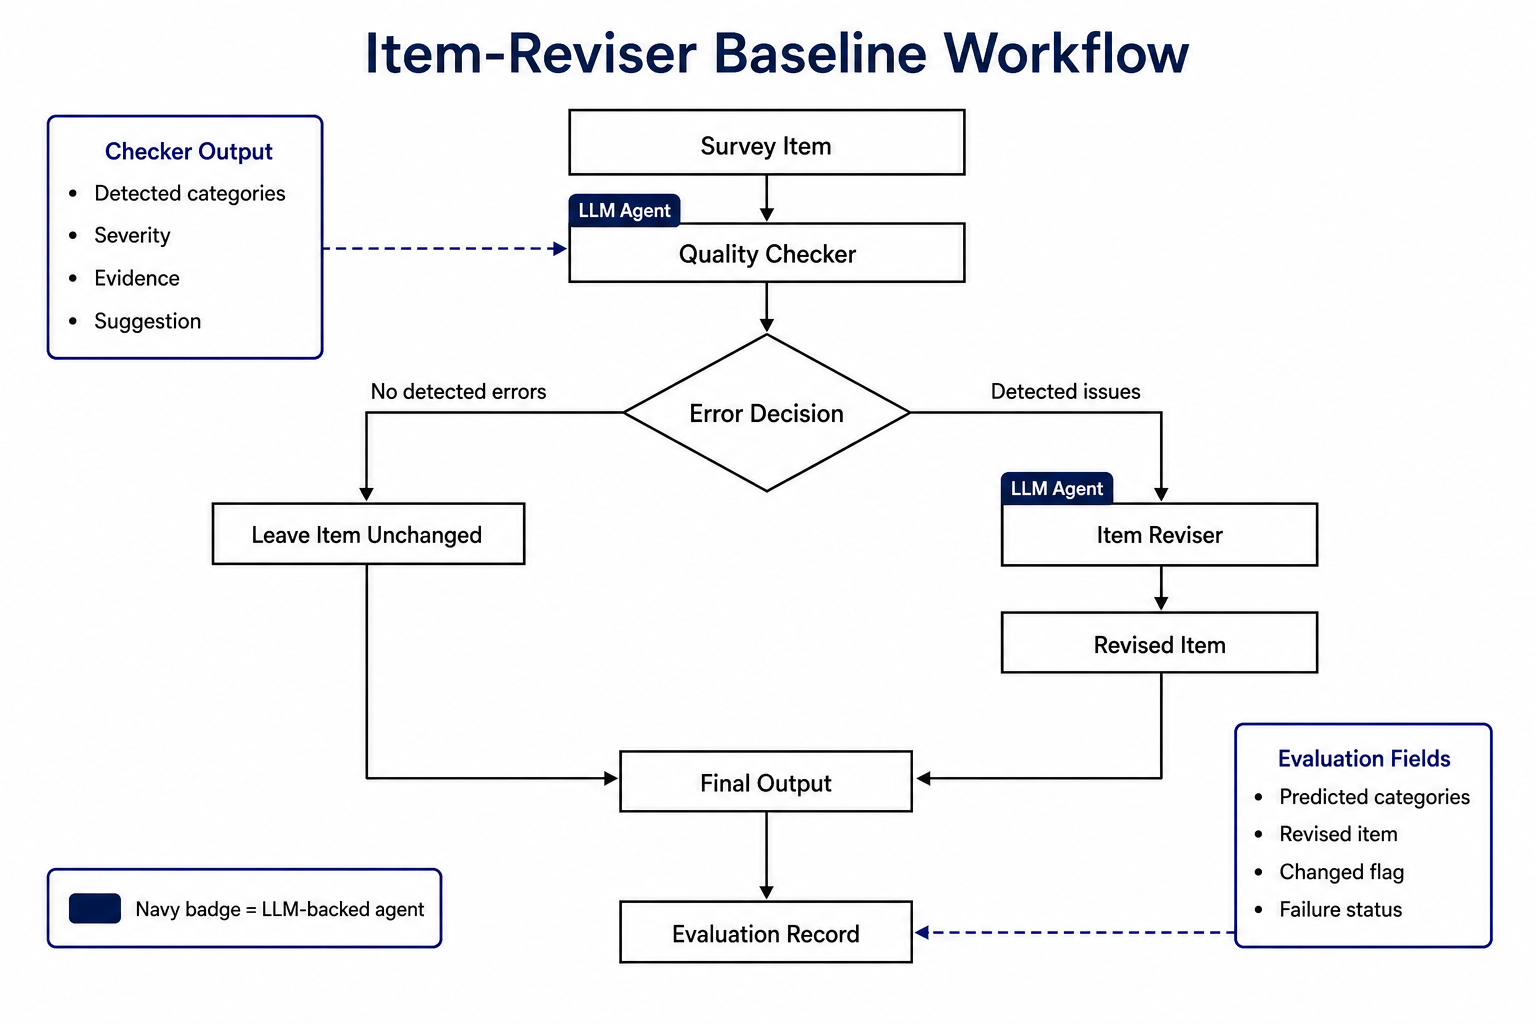
\includegraphics[
        width=0.96\linewidth,
        height=0.47\textheight,
        keepaspectratio
    ]{item_reviser_baseline_agents_academic.png}
    \caption{Baseline workflow with quality checker, item reviser.}
    \label{fig:orchestration}
\end{figure}

\begin{figure}[H]
    \centering
    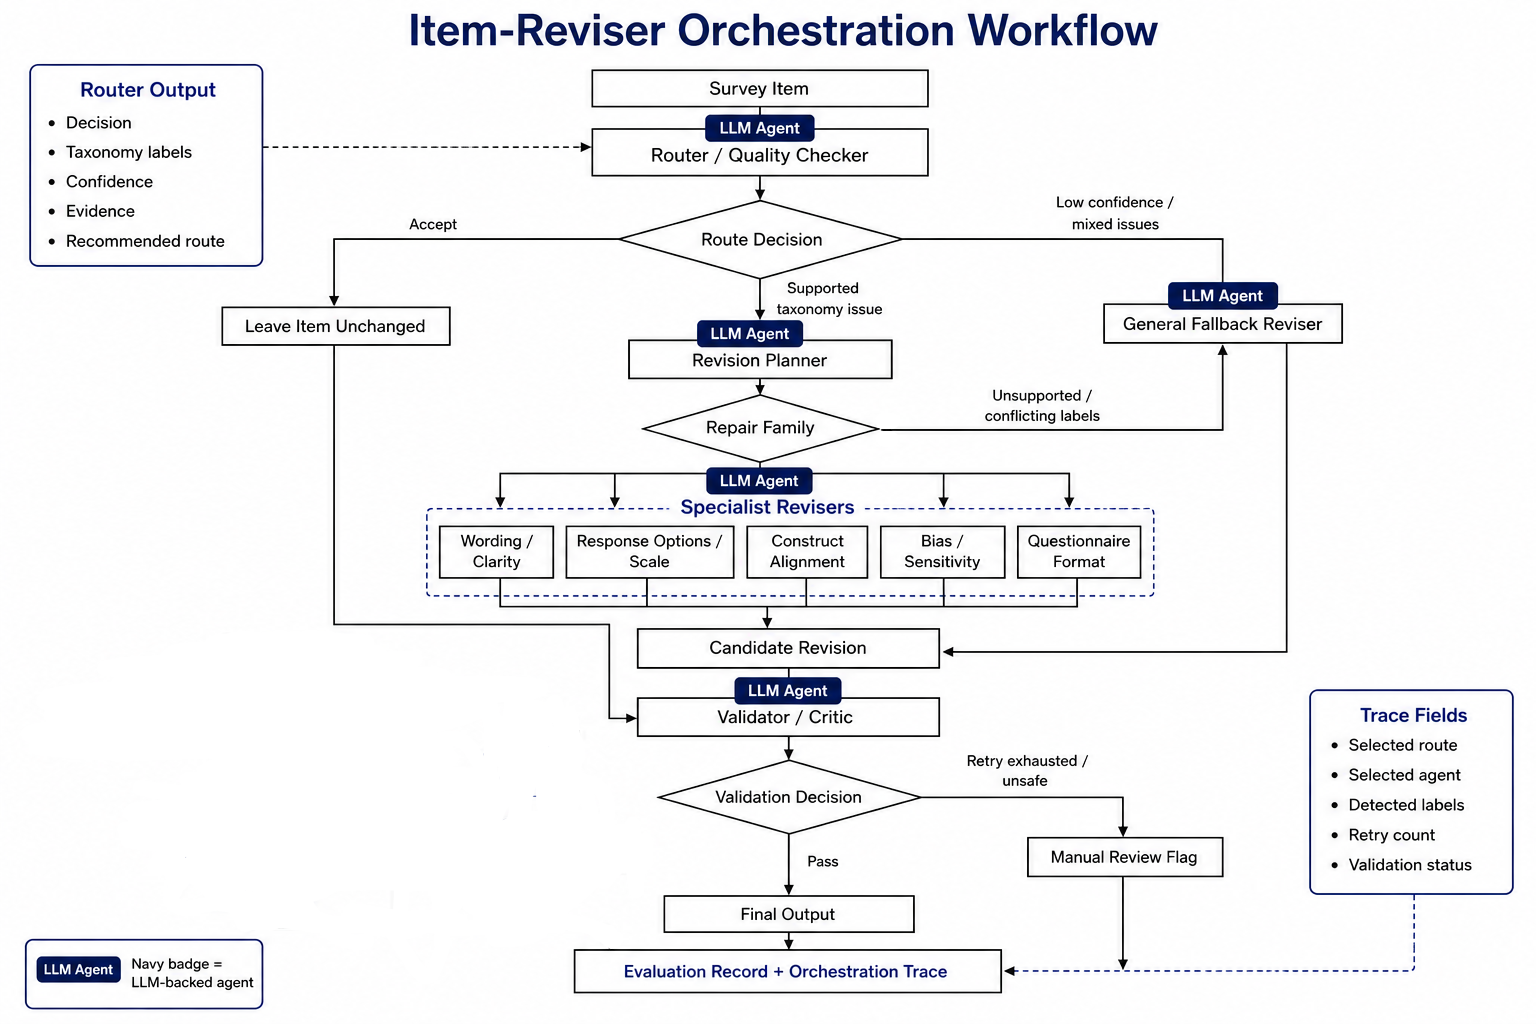
\includegraphics[
        width=0.96\linewidth,
        height=0.47\textheight,
        keepaspectratio
    ]{item_reviser_orchestration_agents_academic.png}
    \caption{Orchestrated workflow with specialist routing, fallback handling,
    validation, and bounded retry.}
    \label{fig:orchestration-agents}
\end{figure}

\clearpage

\section{Supplementary Benchmark Information}
\label{app:benchmark}

\subsection{Benchmark Topic, Format, and Difficulty Coverage}

The benchmark was also designed to reduce dependence on a narrow set of
questionnaire topics. It spans 14 substantive domains, as shown in
Table~\ref{tab:benchmark-topics}. No single topic accounts for more than 19 of
the 200 items.

\begin{table}[H]
\centering
\caption{Topic coverage of the 200-item benchmark.}
\label{tab:benchmark-topics}
\small
\begin{tabularx}{\textwidth}{Xr@{\hspace{2em}}Xr}
\toprule
\textbf{Topic} & \textbf{Count}
& \textbf{Topic} & \textbf{Count}\\
\midrule
Education                 & 19 & Health                    & 19\\
Public services           & 19 & University life           & 16\\
Family/household          & 16 & Technology                & 15\\
Environment               & 15 & Politics/public policy    & 13\\
Mobility                  & 13 & Work                      & 13\\
Media/culture             & 13 & Finances                  & 12\\
Labor                     & 10 & Sensitive behaviors       &  7\\
\bottomrule
\end{tabularx}
\end{table}

Diversity extends beyond subject matter. The items use nine response formats,
including binary yes--no questions, open-ended questions, frequency scales,
numeric ranges, ordinal categories, categorical response sets,
support--oppose scales, agreement scales, and filter questions. The benchmark
also contains three nearly equal difficulty groups: 67 \code{obvious} items,
67 \code{realistic} items, and 66 \code{borderline} items. The obvious cases
contain comparatively salient defects, realistic cases resemble defects that
may occur in ordinary questionnaire development, and borderline cases require
finer distinctions between related taxonomy categories or between an actual
defect and a merely optional improvement.

\subsection{Detailed Comparison with Prior Work}

Table~\ref{tab:related-work-comparison} summarizes the closest lines of work.
The comparison is selective rather than exhaustive and emphasizes differences
in task definition and evaluation design.

\begin{table}[H]
\centering
\caption{Selected questionnaire-evaluation and LLM studies in relation to the
present work.}
\label{tab:related-work-comparison}
\scriptsize
\renewcommand{\arraystretch}{1.12}
\setlength{\tabcolsep}{3.2pt}
\begin{tabularx}{\textwidth}{
    p{0.145\textwidth}
    p{0.165\textwidth}
    p{0.225\textwidth}
    p{0.155\textwidth}
    X
}
\toprule
\textbf{Study/system}
& \textbf{Primary task}
& \textbf{Evaluation basis}
& \textbf{Main output}
& \textbf{Relation to the present study} \\
\midrule

\citet{graesser2006quaid}
& Comprehension screening
& Expert comparisons, assisted revision, and respondent-processing evidence
& Potential comprehension problems
& Automated and actionable, but concentrated on wording, syntax, semantics,
  and memory burden. \\

\citet{saris2014design} / SQP
& Measurement-quality prediction
& MTMM-derived quality estimates and coded formal or linguistic item features
& Predicted reliability, validity, and quality
& Predicts expected quality for supported item types rather than explicit
  defect sets or generated repairs. \\

\citet{adhikari2025exploring}
& Generation, simulated pretesting, and cultural adaptation
& Participant and expert evaluations
& Generated, reviewed, and adapted questionnaire items
& Evaluates a development pipeline rather than gold-taxonomy defect
  classification. \\

\citet{metheney2025generative}
& Prompted critique of existing questions
& 262 questions in a $2\times3$ model--persona experiment; qualitative coding
& Free-text problem statements
& Studies feedback content and prompt effects without a closed gold
  multi-label benchmark. \\

\citet{sturgis2026llms}
& Detection of deliberately embedded flaws
& 20 flawed questions and seven control questions
& Detected problem descriptions
& Includes controls and known flaws, but uses a small benchmark and does not
  systematically evaluate minimal revision. \\

\citet{roberts2026survey}
& Automated QAS-99 appraisal
& 118 draft questions compared with expert and novice coders
& QAS-99 binary appraisal decisions
& Directly evaluates structured appraisal, but not end-to-end generated repair
  or exact multi-label taxonomy recovery. \\

\citet{fuchs2026ai}
& LLM survey-item generation
& Five models, three prompting strategies, and SQP-based evaluation
& Newly generated survey items
& Provides survey-specific evidence that model and prompt choices affect item
  quality. \\

\textbf{Present study}
& \textbf{Defect detection and minimal revision}
& \textbf{200 expert-reviewed items: 40 clean, 115 single-label, and 45
  multi-label}
& \textbf{Taxonomy label set and revised question/options}
& \textbf{Compares models, additive prompt packs, and baseline versus
  orchestrated architectures under one evaluation framework.} \\

\bottomrule
\end{tabularx}
\end{table}

\clearpage
\section{Supplementary Prompt-Pack Information}
\label{app:prompt-packs}

P2 contains 37 fixed, role-specific demonstrations. The role-wise distribution
is reported in Table~\ref{tab:p2-examples}.

\begin{table}[H]
\centering
\caption{Distribution of demonstrations in P2.}
\label{tab:p2-examples}
\small
\begin{tabularx}{0.90\textwidth}{Xr}
\toprule
\textbf{Runtime role} & \textbf{Examples}\\
\midrule
Baseline quality checker / item reviser & 4 / 4\\
Orchestration router & 8\\
Fallback reviser & 3\\
Wording-clarity specialist & 2\\
Response-options-and-scale specialist & 5\\
Construct-alignment specialist & 2\\
Bias-sensitivity specialist & 2\\
Questionnaire-format specialist & 2\\
Validator & 5\\
Revision planner & 0\\
\midrule
\textbf{Total} & \textbf{37}\\
\bottomrule
\end{tabularx}
\end{table}

The router includes at least one example for each specialist family, while the
planner remains zero-shot because it only translates a fixed issue set into the
canonical family and agent. All examples were authored outside the evaluation
benchmark.

\clearpage
\section{Supplementary Detection Results}
\label{app:detection}

\subsection{P0 Cross-Model Family Breakdown}

At P0, Qwen clearly outperformed the other checkpoints. Its baseline F1 of
$0.519$ exceeded Gemma's $0.347$ and Mistral's $0.160$. Under orchestration,
Qwen still reached $0.476$, compared with $0.216$ for Gemma and $0.036$ for
Mistral. The very low clean false-positive rates of the weaker orchestrated
models should not be read as uniformly good performance. Mistral orchestration,
for example, accepted all 40 clean controls but detected only four of the 206
gold-label appearances. Its exact-match rate of $0.205$ was therefore driven
almost entirely by clean items rather than successful defect classification.
Similarly, Gemma P0 orchestration achieved 37 of its 61 exact matches on clean
controls and recovered no multi-label item exactly.

The P0 family results in Table~\ref{tab:p0-cross-model-families} show that the
model differences were not confined to one defect type. Qwen was strongest or
near strongest across all five families. Gemma's baseline result was competitive
for questionnaire format ($F_1=0.870$) and construct alignment ($F_1=0.762$),
but much weaker for response options and scale ($F_1=0.200$). Mistral showed no
true positives for construct alignment or bias sensitivity and only limited
performance in the other families. Orchestration therefore did not compensate
for weak underlying label recognition; it mostly made the weaker models more
conservative.

\begin{table}[H]
\centering
\caption{P0 family-level micro-F1 by model and architecture.}
\label{tab:p0-cross-model-families}
\small
\setlength{\tabcolsep}{4.5pt}
\resizebox{\textwidth}{!}{%
\begin{tabular}{llrrrrr}
\toprule
\textbf{Model} & \textbf{Architecture}
& \textbf{Wording} & \textbf{Construct} & \textbf{Bias}
& \textbf{Format} & \textbf{Options/scale} \\
\midrule
Mistral-7B & Baseline
& 0.140 & 0.000 & 0.000 & 0.154 & 0.208 \\

Mistral-7B & Orchestrated
& 0.100 & 0.000 & 0.000 & 0.000 & 0.000 \\

Gemma-2-9B & Baseline
& 0.343 & 0.762 & 0.444 & 0.870 & 0.200 \\

Gemma-2-9B & Orchestrated
& 0.276 & 0.609 & 0.207 & 0.154 & 0.061 \\

Qwen3.5-9B & Baseline
& 0.469 & 0.917 & 0.682 & 0.556 & 0.488 \\

Qwen3.5-9B & Orchestrated
& 0.495 & 0.857 & 0.667 & 0.286 & 0.350 \\
\bottomrule
\end{tabular}%
}
\end{table}



\subsection{Matched Qwen Detection Counts}

Table~\ref{tab:qwen-detection-counts} reports the complete matched TP, FP, and FN
diagnostics across Qwen prompt packs.

\begin{table}[H]
\centering
\caption{Matched Qwen detection counts and metrics across prompt packs.}
\label{tab:qwen-detection-counts}
\small
\setlength{\tabcolsep}{4.0pt}
\resizebox{\textwidth}{!}{%
\begin{tabular}{llrrrrrrrr}
\toprule
\textbf{Prompt} & \textbf{Architecture}
& \textbf{TP} & \textbf{FP} & \textbf{FN}
& \textbf{Precision} & \textbf{Recall} & \textbf{F1}
& \textbf{Exact} & \textbf{Clean FPR} \\
\midrule
P0 & Baseline
& 136 & 182 & 70 & 0.428 & 0.660 & 0.519 & 0.290 & 0.150 \\

P0 & Orchestrated
& 70 & 18 & 136 & 0.795 & 0.340 & 0.476 & 0.370 & 0.050 \\

P1 & Baseline
& 131 & 186 & 75 & 0.413 & 0.636 & 0.501 & 0.280 & 0.075 \\

P1 & Orchestrated
& 71 & 13 & 135 & 0.845 & 0.345 & 0.490 & 0.375 & 0.025 \\

P2 & Baseline
& 141 & 177 & 65 & 0.443 & 0.684 & 0.538 & 0.270 & 0.175 \\

P2 & Orchestrated
& 87 & 16 & 119 & 0.845 & 0.422 & 0.563 & 0.430 & 0.050 \\
\bottomrule
\end{tabular}%
}
\end{table}

\subsection{Per-Label Qwen Results}

\begin{sloppypar}
Table~\ref{tab:qwen-label-f1} makes the concentration of the P2 effect more
explicit. P2 orchestration substantially improved
\code{leading_question}, \code{loaded_question},
\code{agree_disagree_scale}, \code{incomplete_options},
\code{missing_scale_labels}, and \code{polarity_mismatch}; it also achieved
perfect F1 for \code{too_many_scale_points}. For example, the router changed an
arts-funding item from the incorrect \code{loaded_question} label under P0 and
P1 to the correct \code{leading_question} label under P2. It also began
detecting an agreement-proxy item about drinking-water concern and an unlabeled
confidence scale that P0 and P1 had accepted.

However, several blind spots remained. The orchestrated router produced no true
positives for \code{recall_error}, \code{non_exclusive_options}, or
\code{unbalanced_scale} under any Qwen prompt pack. P2 also reduced
\code{sensitive_topic_direct} and \code{negative_wording} performance relative
to P1 orchestration. This result illustrates the distinction between
family-complete and taxonomy-complete calibration: examples in every family did
not guarantee reliable discrimination for every label within that family.
\end{sloppypar}

\begin{table}[H]
\centering
\caption{Per-label Qwen F1. B and O denote baseline and orchestrated
         architectures.}
\label{tab:qwen-label-f1}
\scriptsize
\setlength{\tabcolsep}{2.8pt}
\resizebox{\textwidth}{!}{%
\begin{tabular}{lrrrrrrr}
\toprule
\textbf{Label} & \textbf{Gold}
& \textbf{P0-B} & \textbf{P0-O}
& \textbf{P1-B} & \textbf{P1-O}
& \textbf{P2-B} & \textbf{P2-O} \\
\midrule
\code{leading_question}
& 12 & 0.595 & 0.600 & 0.537 & 0.857 & 0.585 & 0.957 \\

\code{loaded_question}
& 12 & 0.300 & 0.609 & 0.333 & 0.667 & 0.358 & 0.737 \\

\code{double_barreled}
& 12 & 0.917 & 0.857 & 0.870 & 0.800 & 0.957 & 0.857 \\

\code{recall_error}
& 12 & 0.375 & 0.000 & 0.286 & 0.000 & 0.400 & 0.000 \\

\code{vague_ambiguous}
& 16 & 0.438 & 0.211 & 0.500 & 0.211 & 0.438 & 0.211 \\

\code{sensitive_topic_direct}
& 12 & 0.632 & 0.286 & 0.737 & 0.286 & 0.588 & 0.154 \\

\code{social_desirability}
& 12 & 0.720 & 0.857 & 0.667 & 0.917 & 0.769 & 0.857 \\

\code{negative_wording}
& 13 & 0.889 & 0.783 & 0.815 & 0.727 & 0.857 & 0.667 \\

\code{open_closed_mismatch}
& 12 & 0.556 & 0.286 & 0.632 & 0.400 & 0.471 & 0.400 \\

\code{agree_disagree_scale}
& 13 & 0.526 & 0.000 & 0.435 & 0.111 & 0.615 & 0.435 \\

\code{unbalanced_scale}
& 12 & 0.250 & 0.000 & 0.435 & 0.000 & 0.400 & 0.000 \\

\code{incomplete_options}
& 12 & 0.182 & 0.353 & 0.174 & 0.333 & 0.213 & 0.571 \\

\code{non_exclusive_options}
& 12 & 0.545 & 0.000 & 0.200 & 0.000 & 0.316 & 0.000 \\

\code{missing_scale_labels}
& 20 & 0.811 & 0.000 & 0.800 & 0.000 & 0.872 & 0.261 \\

\code{too_many_scale_points}
& 12 & 0.960 & 0.909 & 0.880 & 0.909 & 0.774 & 1.000 \\

\code{polarity_mismatch}
& 12 & 0.786 & 0.762 & 0.667 & 0.700 & 0.759 & 0.783 \\
\bottomrule
\end{tabular}%
}
\end{table}

A second recurring pattern was systematic baseline overprediction of
\code{incomplete_options} and \code{loaded_question}. Under P0 baseline, these
labels generated 78 and 56 false positives, respectively; under P2 they still
generated 72 and 43. This produced high recall for the labels but very low
precision. Orchestration sharply reduced these false positives, but often did so
by suppressing the label entirely rather than resolving the boundary reliably.
The improvement from P2 orchestration is notable because it increased supported
predictions while retaining this restraint.

\clearpage
\section{Supplementary Revision Results}
\label{app:revision}

Oracle-revision results are shown in
Table~\ref{tab:oracle-revision-results}. For Qwen, P2 increased exact-option
matching from 19 to 23 items in the baseline and from 22 to 23 under
orchestration. Question exact match changed little, and SARI did not improve
consistently. The largest exact-full rate in any complete non-thinking oracle
run was only $0.025$ (4 of 160 items) for Qwen P1 orchestration.

\begin{table}[H]
\centering
\caption{Oracle-revision metrics without thinking. Gold categories are
         supplied, but item-specific evidence and repair suggestions are not.}
\label{tab:oracle-revision-results}
\scriptsize
\setlength{\tabcolsep}{2.8pt}
\resizebox{\textwidth}{!}{%
\begin{tabular}{lllrrrrrrr}
\toprule
\textbf{Model} & \textbf{Prompt} & \textbf{Architecture}
& \textbf{BERTScore} & \textbf{SARI} & \textbf{Exact Q.}
& \textbf{Exact options} & \textbf{Exact full} & \textbf{Changed}
& \textbf{Scored} \\
\midrule
Mistral-7B & P0 & Baseline
& 0.952 & 50.95 & 0.075 & 0.100 & 0.019 & 0.850 & 160/160 \\

Mistral-7B & P0 & Orchestrated
& 0.951 & 58.17 & 0.169 & 0.110 & 0.013 & 1.000 & 154/160 \\

Gemma-2-9B & P0 & Baseline
& 0.953 & 58.30 & 0.087 & 0.100 & 0.013 & 1.000 & 160/160 \\

Gemma-2-9B & P0 & Orchestrated
& 0.955 & 61.70 & 0.180 & 0.107 & 0.013 & 1.000 & 150/160 \\

Qwen3.5-9B & P0 & Baseline
& 0.956 & 62.46 & 0.181 & 0.119 & 0.019 & 0.950 & 160/160 \\

Qwen3.5-9B & P0 & Orchestrated
& 0.956 & 61.94 & 0.194 & 0.138 & 0.019 & 0.950 & 160/160 \\

Qwen3.5-9B & P1 & Baseline
& 0.954 & 61.45 & 0.175 & 0.119 & 0.013 & 0.963 & 160/160 \\

Qwen3.5-9B & P1 & Orchestrated
& 0.956 & 62.02 & 0.188 & 0.138 & 0.025 & 0.944 & 160/160 \\

Qwen3.5-9B & P2 & Baseline
& 0.955 & 61.18 & 0.181 & \textbf{0.144} & 0.019 & 0.825 & 160/160 \\

Qwen3.5-9B & P2 & Orchestrated
& 0.956 & 61.61 & 0.194 & \textbf{0.144} & 0.019 & 0.906 & 160/160 \\
\bottomrule
\end{tabular}%
}
\end{table}

Oracle revision was therefore not a strict empirical upper bound. P2 baseline
left 28 gold-flawed items unchanged and P2 orchestration left 15 unchanged,
despite receiving the correct categories. Inspection of the revision notes
showed that the revisers sometimes rejected a gold label because the oracle
issue object contained \code{evidence=null}. For example, some
\code{loaded_question} items were preserved because a premise-denial option was
interpreted as sufficient evidence that no stem repair was needed. This behavior
follows the prompts' conservative evidence gate, but it means that oracle mode
measures revision from correct label-only guidance rather than revision from a
fully specified expert diagnosis. It also explains why oracle scores did not
consistently exceed end-to-end scores. The 40 clean controls are preserved
unchanged by construction in oracle mode and are excluded from the revision
averages; their perfect preservation is not treated as model performance.

\clearpage
\section{Supplementary Thinking-Mode Results}
\label{app:thinking}

\subsection{Completion Reliability}

Table~\ref{tab:thinking-completion} separates items reached, successful
structured outputs, failed outputs, and unprocessed rows. The end-to-end
baseline produced only 57 successful outputs and the orchestrated version 62.
The baseline oracle run reached all items but failed on 56; the orchestrated
oracle run stopped after 128 items. Token exhaustion was the main operational
cause: the model often consumed the generation budget on internal reasoning and
then returned truncated, empty, or schema-invalid JSON.

\begin{table}[H]
\centering
\caption{Thinking-mode completion. The final column gives successful clean,
         single-label, and multi-label items.}
\label{tab:thinking-completion}
\small
\setlength{\tabcolsep}{4.0pt}
\resizebox{\textwidth}{!}{%
\begin{tabular}{llrrrrc}
\toprule
\textbf{Architecture} & \textbf{Mode} & \textbf{Reached}
& \textbf{Successful} & \textbf{Failed} & \textbf{Unprocessed}
& \textbf{Successful C/S/M} \\
\midrule
Baseline
& End-to-end & 149 & 57 & 92 & 51 & 21/33/3 \\

Baseline
& Oracle & 200 & 144 & 56 & 0 & 40/74/30 \\

Orchestrated
& End-to-end & 138 & 62 & 76 & 62 & 19/42/1 \\

Orchestrated
& Oracle & 128 & 92 & 36 & 72 & 40/52/0 \\
\bottomrule
\end{tabular}%
}
\end{table}

\subsection{Conditional Revision Result}

Only the baseline oracle thinking run produced final semantic revision metrics.
Table~\ref{tab:thinking-conditional-revision} reports them conditionally on the
104 successful flawed items. Exact-option matching reached 22 of 104 items
($0.212$), but no comparison is made with a full non-thinking run because that
would use a different item set. A matched-subset semantic rescore was not
contained in the archived artifacts.

\begin{table}[H]
\centering
\caption{Conditional revision quality for the completed P2 baseline-oracle
         thinking outputs.}
\label{tab:thinking-conditional-revision}
\small
\begin{tabular}{lrrrrrr}
\toprule
\textbf{Scored} & \textbf{BERTScore} & \textbf{SARI}
& \textbf{Exact Q.} & \textbf{Exact options} & \textbf{Exact full}
& \textbf{Changed} \\
\midrule
104/160 & 0.958 & 63.47 & 0.154 & 0.212 & 0.048 & 1.000 \\
\bottomrule
\end{tabular}
\end{table}

\clearpage
\section{Exploratory Semantic Option Matching Metric}
\label{app:som-f1}

This appendix outlines a proposed, exploratory metric that was not used in the
experiments reported in this paper.

A further direction concerns evaluation of response-option revisions. Exact
option matching is intentionally transparent but very strict. Semantically
equivalent revisions such as ``Very dissatisfied'' and ``Very unhappy'' receive
no credit unless their normalized strings are identical. An exploratory
\emph{Semantic Option Matching F1} (SOM-F1) could address this limitation while
still penalizing missing and additional options. For gold option set $E$ and
predicted option set $P$, a semantic model would score all predicted--gold
option pairs and optimal one-to-one matching would be obtained with the
Hungarian algorithm. If $M$ denotes the resulting matching and $s(e,p)$ the
semantic similarity of a matched pair, the metric would be

\[
P_{\mathrm{sem}}
=
\frac{\sum_{(e,p)\in M}s(e,p)}{|P|},
\qquad
R_{\mathrm{sem}}
=
\frac{\sum_{(e,p)\in M}s(e,p)}{|E|},
\]

\[
\mathrm{SOM}\text{-}F1
=
\frac{2P_{\mathrm{sem}}R_{\mathrm{sem}}}
     {P_{\mathrm{sem}}+R_{\mathrm{sem}}}.
\]

A defensible implementation would use a
pretrained cross-encoder, preferably one trained for natural-language
inference. Bidirectional entailment could provide evidence that two options
express approximately the same response meaning, while high contradiction
probability could prevent opposite-polarity options such as ``Very satisfied''
and ``Very dissatisfied'' from receiving misleadingly high similarity.

Before SOM-F1 could be used as a research metric, it would require an
independent human-labelled validation set containing synonymous options,
opposite polarities, neutral categories, frequency and quantity scales, numeric
ranges, residual options, and missing or additional categories. Model selection
and calibration should be performed only on development pairs, followed by
evaluation on held-out pairs.
\end{document}
